%!TEX root = FreeRtos ARM uController.tex
\subsection{Komplexität durch Nebenläufigkeit - Debugging von Echtzeitsystemen}
\label{sec:Debugging von Echtzeitsystemen}
Durch den Einsatz eines Echtzeitbetriebssystems erhält der Entwickler einige Vorteile, die bereits in Abschnitt \ref{sec:Echtzeitsysteme} beschrieben wurden. Im Gegenzug entstehen aber durch die Nebenläufigkeit neue mögliche Fehlerquellen. Viele dieser Fehler lassen sich nicht einfach analysieren und enden oft im HardFault Handler. Der HardFault Handler ist dabei eine Art Endstation und wird aufgerufen, sobald der $\mu$Prozessor feststellt, dass eine schwerwiegende, fehlerhafte Operation stattgefunden hat. Des Weiteren können na\-tür\-lich auch gewöhnliche Synchronisationsprobleme auftreten, wie Starvation oder Deadlocks. Dieser Abschnitt soll dabei nicht erklären wie solche Probleme im Detail gelöst werden können, dies wir bereits hinlänglich in der Literatur behandelt z.B. in \cite{9783827373427} \cite{9783864902222}. Dieser Abschnitt soll zeigen, welche Tools und Möglichkeiten ein Entwickler hat, um solche Probleme ausfindig zum machen. Beim Debuggen einer Anwendung kann der Entwickler gewöhnlich durch die Nutzung eines ISPs auf die aktuellen Registerinhalte und den Stack des $\mu$Prozessors zugreifen. 
%Ist stack hier Singular oder Plural?
Das Problem ist, dass eine FreeRTOS Anwendung gewöhnlich aus mehreren Task besteht und jede Task eine eigene Anwendungseinheit darstellt. Der Stack und die Register einer verdrängten Task werden durch das Echtzeitbetriebssystem gesichert und sind für den ISP nicht mehr sichtbar. Daher bieten einige ISP Hersteller spezielle Thread Aware Pakete. Diese ermöglichen das Auslesen von Daten einer blockierten Task, siehe Abbildung \ref{fig:ThreadAware}.
\begin{figure}[hbt]
	\centering
		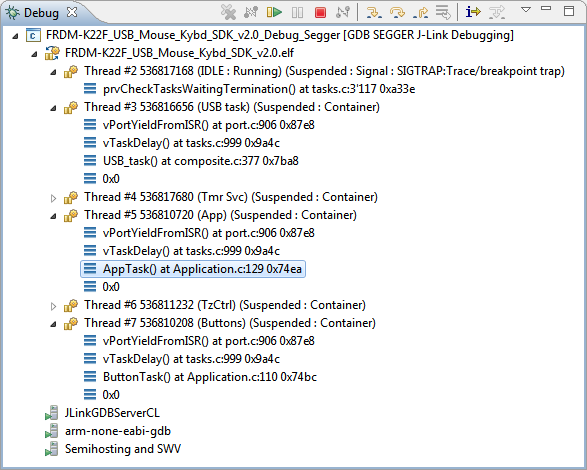
\includegraphics[width=0.5\textwidth]{Pictures/Segger/freertosThreadAwareness}
	\caption{In diesem Beispiel ist die IDLE Task running, alle anderen Task blockieren (Hier wird für den Zustand Blocked die Bezeichnung Suspended verwendet). Es kann jedoch durch die Thread Awareness auf den Stacktrace der anderen Task zugegriffen werden }
	\label{fig:ThreadAware}
\end{figure}
Ein weiteres, sehr mächtiges Tool zur Analyse von Anwendungen, die auf einem Echtzeitbetriebssystem aufsetzen, sind die sogenannten Trace Tools. Diese ermöglichen die Aufnahme der Scheduling Vorgänge zur Programmlaufzeit, wie in Abbildung \ref {fig:Systemview} dargestellt. 
\begin{figure}[hbt]
	\centering
		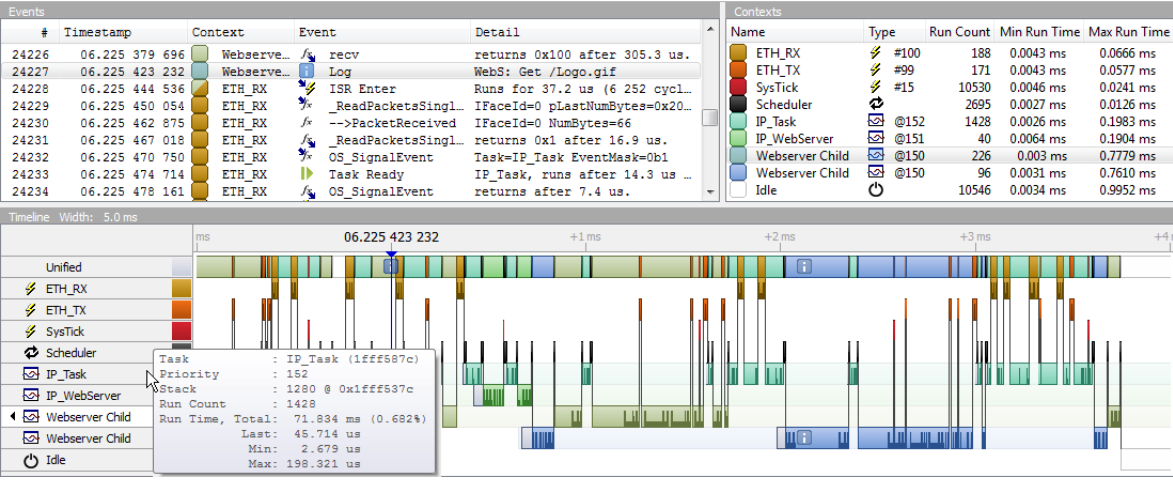
\includegraphics[width=0.5\textwidth]{Pictures/Segger/systemview.png}
	\caption{Trace Tool Segger Systemview ermöglicht die Aufnahme aller Schedulingvorgänge und stellt diese im zeitlichen Verlauf dar. Dem Entwickler ist es somit möglich alle RTOS Operationen rückblickend zu betrachten.}
	\label{fig:Systemview}
\end{figure}
Besonders in Anwendungen, in den viele Tasks interagieren, ist der Einsatz eines solchen Tools fast unabdingbar. Viele dieser Trace Tools ermöglichen eine ununterbrochene Aufzeichnung des RTOS Kernels. Besonders Fehler, die erst nach sehr langer Programmlaufzeit auftreten oder aber nur sporadisch stattfinden, können so entdeckt und analysiert werden. Für die Nutzung von Trace Tools werden weitere Bibliotheken benötigt, die eine weitere Schicht zwischen Hardware und Echtzeitbetriebssystem bilden, siehe Abbildung \ref{fig:SystemviewTarget}. Eine noch bessere Möglichkeit zum Aufzeichnen der Vorgänge auf dem embedded System, sind die sogenannten Trace Recorder. Dabei handelt es sich um ISP Programmer mit integriertem Trace Buffer (z.B. Segger J-Trace). Mit einem Trace Recorder kann der gesamte Programmablauf aufgenommen werden. Der Trace Rekorder nimmt nicht nur FreeRTOS spezifische Abläufe auf, sondern alle Instruktionen des $\mu$Prozessors. Dadurch ist es möglich rückwärts durch den Instruktionsverlauf zu springen. Man kann die Anwendung also quasi zurückspulen.
\begin{figure}[hbt]
	\centering
		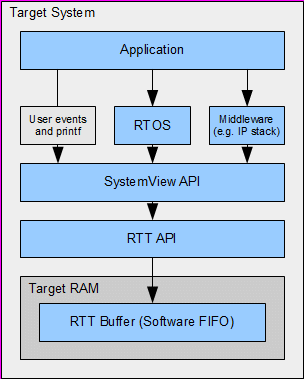
\includegraphics[width=0.4\textwidth]{Pictures/Segger/SystemViewTarget.png}
	\caption{Die benötigten Target Files für die Trace Tools bilden eine weitere Middleware Schicht.}
	\label{fig:SystemviewTarget}
\end{figure}
